\documentclass[12pt]{article} 

% --- Layout ---
\usepackage[a4paper, margin=1in]{geometry} 
\usepackage{parskip}  
\usepackage{setspace} 
\usepackage{graphicx}
\onehalfspacing       

% --- Font ---
\usepackage{lmodern}  
\usepackage[T1]{fontenc}

% --- Math Packages ---
\usepackage{mathtools}
\allowdisplaybreaks


\begin{document}

\title{\Huge Lagrange Method I}
\author{Jerry Wu}
\date{}
\maketitle

\begin{figure}[h]
    \centering
    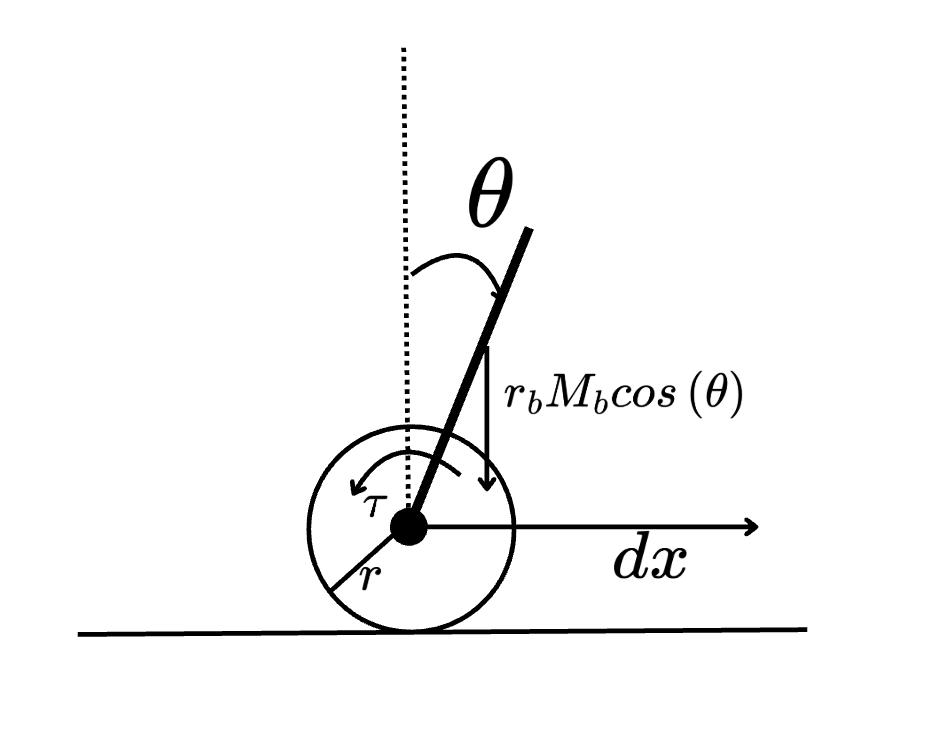
\includegraphics[width=0.5\textwidth]{Lagrange_Diagram.png}
    \caption{Lagrange Method 1 Diagram}
    \label{fig:your-label}
\end{figure}

\section*{Define Lagrange}
\begin{multline*}
T= 0.5 I_{b} \dot{\phi}^{2} + \frac{0.5 I_{w} \dot{x}^{2}}{r^{2}} + 0.5 M_{b} \left(L_{b}^{2} \dot{\phi}^{2} + 2 L_{b} \dot{\phi} \dot{x} \cos{\left(\phi \right)} + \dot{x}^{2}\right) + 0.5 M_{w} \dot{x}^{2}
\end{multline*}
\begin{multline*}
T= L_{b} M_{b} g \cos{\left(\phi \right)}
\end{multline*}
\begin{multline*}
L= 0.5 I_{b} \dot{\phi}^{2} + \frac{0.5 I_{w} \dot{x}^{2}}{r^{2}} - L_{b} M_{b} g \cos{\left(\phi \right)} + 0.5 M_{b} \left(L_{b}^{2} \dot{\phi}^{2} + 2 L_{b} \dot{\phi} \dot{x} \cos{\left(\phi \right)} + \dot{x}^{2}\right) + 0.5 M_{w} \dot{x}^{2}
\end{multline*}

\section*{X Coordinate}
\begin{multline*}
\frac{\partial L}{\partial \dot{x}}= \dot{\phi} \left(\frac{I_{b}}{r} + \frac{L_{b}^{2} M_{b}}{r} + L_{b} M_{b} \cos{\left(\phi \right)}\right) + \dot{x} \left(\frac{I_{w}}{r^{2}} + \frac{L_{b} M_{b} \cos{\left(\phi \right)}}{r} + M_{b} + M_{w}\right)
\end{multline*}
\begin{multline*}
\frac{d}{dt}(\frac{\partial L}{\partial \dot{x}})= - L_{b} M_{b} \dot{\phi}^{2} \sin{\left(\phi \right)} - \frac{L_{b} M_{b} \dot{\phi} \dot{x} \sin{\left(\phi \right)}}{r} \\
+ \ddot{\phi} \left(\frac{I_{b}}{r} + \frac{L_{b}^{2} M_{b}}{r} + L_{b} M_{b} \cos{\left(\phi \right)}\right) + \ddot{x} \left(\frac{I_{w}}{r^{2}} + \frac{L_{b} M_{b} \cos{\left(\phi \right)}}{r} + M_{b} + M_{w}\right)
\end{multline*}
\begin{multline*}
\frac{\partial L}{\partial x}= - \frac{L_{b} M_{b} \dot{\phi} \dot{x} \sin{\left(\phi \right)}}{r} + \frac{L_{b} M_{b} g \sin{\left(\phi \right)}}{r}
\end{multline*}

\begin{multline*}
- L_{b} M_{b} \dot{\phi}^{2} \sin{\left(\phi \right)} - \frac{L_{b} M_{b} g \sin{\left(\phi \right)}}{r} + \ddot{\phi} \left(\frac{I_{b}}{r} + \frac{L_{b}^{2} M_{b}}{r} + L_{b} M_{b} \cos{\left(\phi \right)}\right)\\
+ \ddot{x} \left(\frac{I_{w}}{r^{2}} + \frac{L_{b} M_{b} \cos{\left(\phi \right)}}{r} + M_{b} + M_{w}\right)=-\frac{\tau}{r}
\end{multline*}

\section*{$\theta$ Coordinate}
\begin{multline*}
\frac{\partial L}{\partial \dot{\theta}}= \dot{\phi} \left(I_{b} + L_{b}^{2} M_{b}\right) + \dot{x} L_{b} M_{b} \cos{\left(\phi \right)}
\end{multline*}
\begin{multline*}
\frac{d}{dt}(\frac{\partial L}{\partial \dot{\theta}})= - L_{b} M_{b} \dot{\phi} \dot{x} \sin{\left(\phi \right)} + \ddot{\phi} \left(I_{b} + L_{b}^{2} M_{b}\right) + \ddot{x} L_{b} M_{b} \cos{\left(\phi \right)}
\end{multline*}
\begin{multline*}
\frac{\partial L}{\partial \theta}= - L_{b} M_{b} \dot{\phi} \dot{x} \sin{\left(\phi \right)} + L_{b} M_{b} g \sin{\left(\phi \right)}
\end{multline*}
\begin{multline*}
- L_{b} M_{b} g \sin{\left(\phi \right)} + \ddot{\phi} \left(I_{b} + L_{b}^{2} M_{b}\right) + \ddot{x}L_{b} M_{b} \cos{\left(\phi \right)}=\tau
\end{multline*}


\section*{Solve The Equation(By Sympy)}
\begin{multline*}
\ddot{x}= \frac{I_{b} M_{b} \dot{\theta}^{2} r^{2} r_{b} \sin{\left(\theta \right)}}{D} \\
- \frac{I_{b} r \tau}{D} + \frac{M_{b}^{2} \dot{\theta}^{2} r^{2} r_{b}^{3} \sin{\left(\theta \right)}}{D} - \frac{M_{b}^{2} g r^{2} r_{b}^{2} \sin{\left(\theta \right)} \cos{\left(\theta \right)}}{D} - \frac{M_{b} r^{2} r_{b} \tau \cos{\left(\theta \right)}}{D} \\
- \frac{M_{b} r r_{b}^{2} \tau}{D}
\end{multline*}

\begin{multline*}
\ddot{\theta} = 
\ddot{\theta}= \frac{I_{w} M_{b} g r_{b} \sin{\left(\theta \right)}}{D} + \frac{I_{w} \tau}{D} - \frac{M_{b}^{2} \dot{\theta}^{2} r^{2} r_{b}^{2} \sin{\left(\theta \right)} \cos{\left(\theta \right)}}{D} \\
+ \frac{M_{b}^{2} g r^{2} r_{b} \sin{\left(\theta \right)}}{D} + \frac{M_{b} M_{w} g r^{2} r_{b} \sin{\left(\theta \right)}}{D} + \frac{M_{b} r^{2} \tau}{D} + \frac{M_{b} r r_{b} \tau \cos{\left(\theta \right)}}{D} + \frac{M_{w} r^{2} \tau}{D}
\end{multline*}

\[
D = I_{b} I_{w} + I_{b} M_{b} r^{2} + I_{b} M_{w} r^{2} + I_{w} M_{b} r_{b}^{2} - M_{b}^{2} r^{2} r_{b}^{2} \cos^{2}{\left(\theta \right)} + M_{b}^{2} r^{2} r_{b}^{2} + M_{b} M_{w} r^{2} r_{b}^{2}
\]

\section*{Linearized System}
\begin{align*}
    \mathbf{A} &=
    \begin{bmatrix}
    0 & 1 & 0 & 0 \\[10pt]
    0 & 0 & -\dfrac{M_b^2 g r^2 r_b^2}{D} & 0 \\[10pt]
    0 & 0 & 0 & 1 \\[10pt]
    0 & 0 & \dfrac{I_w M_b g r_b + M_b^2 g r^2 r_b + M_b M_w g r^2 r_b}{D} & 0
    \end{bmatrix} \\[16pt]
    %
    \mathbf{B} &=
    \begin{bmatrix}
    0 \\[10pt]
    - \dfrac{I_b r + M_b r^2 r_b + M_b r r_b^2}{D} \\[10pt]
    0 \\[10pt]
    \dfrac{I_w + M_b r^2 + M_b r r_b + M_w r^2}{D}
    \end{bmatrix} \\[16pt]
    %
    \text{where} \quad
    D &= I_b I_w + I_b M_b r^2 + I_b M_w r^2 + I_w M_b r_b^2 + M_b M_w r^2 r_b^2
\end{align*}
    
  

\end{document}
